\documentclass[12pt,a4paper]{article}
\usepackage[utf8x]{inputenc}
\usepackage[english,hebrew]{babel}
\selectlanguage{hebrew}
\usepackage{graphicx}
\usepackage{verbatim}
\usepackage{url}

\graphicspath{{images/}}

\usepackage{tikz}
\usetikzlibrary{external,positioning,through,calc,intersections,arrows.meta}
\tikzexternalize[prefix=tikz/]

\textwidth=15cm
\textheight=23cm
\topmargin=0pt
\headheight=0pt
\oddsidemargin=2em
\headsep=0pt
\parindent=0pt

\begin{document}
\thispagestyle{empty}

\begin{center}
\textbf{\Huge שגיאות בפתרון שאלות במתמטיקה}

\bigskip
\bigskip

\textbf{\Large מוטי בן-ארי}

\bigskip

\textbf{\Large המחלקה להוראת המדעים}

\bigskip

\textbf{\Large מכון ויצמן למדע}

\end{center}

\bigskip

\selectlanguage{english}

\begin{center}
\copyright{}\  2016--17 by Moti Ben-Ari.
\end{center}

This work is licensed under the Creative Commons Attribution-ShareAlike 3.0 Unported License. To view a copy of this license, visit \url{http://creativecommons.org/licenses/by-sa/3.0/} or send a letter to Creative Commons, 444 Castro Street, Suite 900, Mountain View, California, 94041, USA.

\bigskip

\begin{center}

\includegraphics[width=.2\textwidth]{../by-sa.png}
\end{center}

\selectlanguage{hebrew}

\section*{מבוא}


העוסקים במתמטיקה שוגים ומנסים דרכי פתרון שמובילות למבוי סתום! בספרים מופיעים שכתובים נקיים ומסודרים של ההוכחות והחישובים ולא את ערימות הנייר שנזרקו לפח בדרך. לדעתי, חשוב לראות בשגיאה לא סימן לכישלון אלא אתגר שיש להתמודד איתו.

\bigskip

במסמך זה אביא פתרונות לשאלות מבחינות הבגרות במתמטיקה )שאלון
$806$,
תשע"ד ותשע"ה( פחות או יותר כפי שפתרתי כולל שגיאות. לאחר ההתאוששות מהשגיאה אדון במאפייני השגיאה.


\begin{center}
* * *
\end{center}

ברצוני להודות לרונית בן-בסט לוי ולאביטל אלבוים-כהן שקראו את המסמך והעירו הערות מועילות. במקרים מסויימים הן הציעו דרכי פתרון אחרות. לא שניתי את דרכי הפתרון שלי כדי לשמור על "אוטנטיות", ולכן שילבתי את הצעותיהן בסעיפי "המסקנות".

\newpage

%%%%%%%%%%%%%%%%%%%%%%%%%%%%%%%%%%%%%%%%%%%

\section*{קיץ תשע"ה מועד ב, שאלה 1}

\begin{center}
\selectlanguage{english}
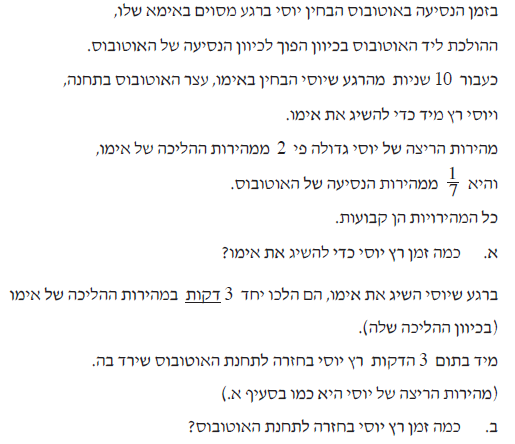
\includegraphics[width=.8\textwidth]{summer-2015b-1}
\end{center}

\vspace{-4ex}\paragraph{סעיף א}
\mbox{}

\textbf{תרשים תנועה}
\begin{center}
\selectlanguage{english}
\begin{tikzpicture}
\draw[dashed,->] (0,1) node[above] {
\R{מפגש ראשון}
} -- (0,.2);
\draw[dashed,->] (-3,1) node[yshift=1pt,above] {
\R{מפגש שני}
} -- (-3,.2);
\draw[->] (0,0) -- node[above] {
\R{יוסי אוטובוס}
} (4,0);
\draw[->] (0,0) -- node[above] {
\R{אמא}
} (-3,0);
\draw[fill] (0,0) circle [radius=1pt];
\draw[->] (4,-1) -- node[above] {
\R{יוסי ריצה}
} (-3,-1);
\path (0,-1) -- (0,-1.1);
\end{tikzpicture}
\end{center}

המפגש הראשון הוא הנקודה בה יוסי יושב באוטובוס ורואה את אימו. הוא נוסע ימינה עד התחנה ואז רץ שמאלה כדי להשיג את אימו במפגש השני.

\medskip

\textbf{סימונים}

מהירויות: אמא $v_e$, יוסי בריצה $v_r$, יוסי באוטובוס $v_a$.

זמנים: אמא $t_e$, יוסי בריצה $t_r$, יוסי באוטובוס $t_a$.

\pagebreak[3]

\textbf{פתרון}

המרחק שיוסי רץ שווה לסכום המרחקים שאמו הולכת ושל נסיעתו באוטובוס:
\selectlanguage{english}
\begin{equation}
v_r t_r = v_e t_e + v_a t_a\,. \label{e.v}
\end{equation}
\selectlanguage{hebrew}
נתון: יוסי משיג את אמא לאחר פרק הזמן בו שנסע באוטובוס וגם רץ:
\selectlanguage{english}
\begin{equation}
t_e = t_a + t_r\,. \label{e.t}
\end{equation}
\selectlanguage{hebrew}
נתון יחסי המהירויות:
\[
v_r = 2v_e = v_a/7\,.
\]
שנציב עבור
$v_e, v_a$
במשוואה
\L{(\ref{e.v})}:
\begin{eqnarray*}
v_r t_r &=& v_e t_e + v_a t_a\\
v_r t_r &=& \frac{v_r}{2} t_e + 7v_r t_a\\
t_r &=& \frac{t_e}{2}+ 7t_a\\\
t_e &=& -14t_a + 2t_r\,.
\end{eqnarray*}
ביחד עם משוואה
\L{(\ref{e.t})}
 יש לנו שתי נוסחאות עבור
$t_e$:
\[
t_a + t_r = t_e = -14t_a + 2t_r
\]

נתון נוסף הוא שזמן הנסיעה באוטובוס
$t_a$
שווה ל-
$10$
שניות. לכן: 
\begin{eqnarray*}
10+t_r &=& -140 + 2t_r\\
t_r &=& 150\,.
\end{eqnarray*}


\vspace{-4ex}\paragraph{סעיף ב}

נתון: יוסי הולך ביחד עם אמו ובקצב שלה למשך
$3$
דקות. מכאן שהמרחק שהלכו הוא
$3v_e$.
כדי לחזור לתחנת האוטובוס, יוסי חייב לרוץ מרחק זה ועוד המרחק שרץ קודם כדי להשיג את אמו שהוא
$150v_4$.
נסמן ב-
$t_h$
את הזמן שיוסי רץ בהחזרה. נרכיב את הכל הנתונים ונקבל:
\begin{eqnarray*}
t_h &=& \frac{3v_e + 150v_r}{v_r}\\
&=& 150 + \frac{3v_e}{v_r}\\
&=& 150 + \frac{3v_e}{2v_e}\\
&=& 151.5\,.
\end{eqnarray*}

\vspace{-4ex}\paragraph{שגיאה!}
משהו לא הגיוני. רק עוד
$1.5$
שניות? עיון חוזר בשאלה מגלה שהם הלכו ביחד
$3$
\textbf{\R{דקות}}
שהן
$180$
שניות. לכן התשובה הנכונה היא:
\[
t_h = 150 + \frac{180\cdot v_e}{2v_e} = 240\,.
\]
\vspace{-4ex}\paragraph{עבדנו קשה מדי}

הזמן שיוסי רץ מורכב מהזמן לחזור לנקודת המפגש ועוד הזמן מהמפגש לתחנה. אבל כבר חישבנו שהזמן לחזור מהמפגש לתחנה הוא
$150$
שניות. למספר זה נחבר את הזמן הדרוש לרוץ את המרחק שהלכו ביחד במשך שלוש דקות. מהירות הריצה היא פי שנים ממהירות ההליכה, ולכן
$t_h = 150 + 180/2 = 240$.

\paragraph{מסקנות}

\begin{itemize}
\item
\textbf{\R{קרא בעיון את השאלה}}.
כל מילה חשובה. כאן יש מוקש בהחלפת היחידות משניות לדקות אבל המוקש מודגש וניתן לנחש שלהדגשה יש משמעות!

\item
פתרתי את חלק ב' בצורה מסובכת מדי. ייתכן שהייתי שם לב לדרך הפשוטה לו טרחתי לעדכן את תרשים התנועה:
\begin{center}
\selectlanguage{english}
\begin{tikzpicture}
\draw[dashed,->] (0,1) node[above] {
\R{מפגש ראשון}
} -- (0,.1);
\draw[dashed,->] (-3,1) node[yshift=1pt,above] {
\R{מפגש שני}
} -- (-3,0);
\draw[dashed,->] (-6,1) node[yshift=1pt,above] {
\R{נקודת פנייה}
} -- (-6,-2);
\draw[->] (0,0) -- node[above] {
\R{יוסי אוטובוס}
} (4,0);
\draw[->] (0,0) -- node[above] {
\R{אמא}
} (-3,0);
\draw[fill] (0,0) circle [radius=1pt];
\draw[->] (4,-1) -- node[above] {
\R{יוסי ריצה}
} (-3,-1);
\path (0,-1) -- (0,-1.1);
\draw[->] (-3,0) -- node[above] {
\R{הליכה ביחד}
} (-6,0);
\draw[<-,dashed] (-3,0) -- (-3,-1);
\draw[->,dashed] (-6,-3) -- node[above] {
\textbf{\R{ריצה נוספת בחרזה}}
} (-3,-3);
\draw[->] (-6,-2) -- node[above] {
\R{יוסי ריצה בחזרה}
} (4,-2);
\path (0,-3.1) rectangle (5,.1);
\end{tikzpicture}
\end{center}
בתרשים המורחב, יוסי מצטרף לאמו במפגש השני והם הולכים ביחד בקצב הליכה של אמו עד לנקודת הפנייה חזרה של יוסי. כמובן  שהמרחק מנקודת הפנייה עד למפגש השני שווה למרחק מהמפגש השני ועד לנקודת הפנייה.
\item
אפשר להפריד את המסלולים של יוסי ושל אימו בתרשים התנועה:
\begin{center}
\selectlanguage{english}
\begin{tikzpicture}
\draw[dashed,->] (0,2) node[above] {
\R{מפגש ראשון}
} -- (0,.2);
\draw[dashed,->] (-3,2) node[yshift=1pt,above] {
\R{מפגש שני}
} -- (-3,-.9);
\draw[->] (0,0) -- node[above] {
\R{יוסי אוטובוס}
} (4,0);
\draw[->] (0,1) -- node[above] {
\R{אמא}
} (-3,1);
\draw[fill] (0,0) circle [radius=1pt];
\draw[fill] (0,1) circle [radius=1pt];
\draw[fill] (4,-1) circle [radius=1pt];
\draw[->] (4,-1) -- node[above] {
\R{יוסי ריצה}
} (-3,-1);
\path (0,-1) -- (0,-1.1);
\end{tikzpicture}
\end{center}

\item
מקובל לארגן את הנתונים בטבלה:

\begin{center}
\renewcommand{\arraystretch}{1.2}
\setlength{\tabcolsep}{12pt}
\begin{tabular}{|c|c|c|c|}
\hline
\R{מרחק}&\R{מהירות}&\R{זמן}&\\
\R{ק"מ}&\R{ק"מ לשניה}&\R{שניות}&\\\hline
$140v$&$14v$&$10$&\R{יוסי אוטובוס}\\\hline
$2vt$&$2v$&$t$&\R{יוסי ריצה}\\\hline
$v(t+10)$&$v$&$t+10$&\R{אימא}\\\hline
\end{tabular}
\end{center}


\end{itemize}

\newpage

\noindent\textbf{
תרשים תנועה דו-ממיד
}

\medskip

ניתן לפתור את הבעיה בקלות אם נסתייע בתרשים דו-ממדי של התנועה, כאשר הציר האופקי הוא זמן והציר האנכי הוא מרחק:
\begin{center}
\selectlanguage{english}
\begin{tikzpicture}[scale=.95]
\draw (0,0) -- (14,0);
\draw (0,-4) node[left] {
\R{פרידה}
} -- (0,-2) node[left] {
\R{מפגש 2}
} -- (0,0) node[left] {
\R{מפגש 1}
} -- (0,4) node[left] {
\R{תחנה}
};
\fill (0,0) circle [radius=2pt];
\fill (1,0) circle [radius=2pt];
\fill (4,0) circle [radius=2pt];
\fill (8,0) circle [radius=2pt];
\fill (11,0) circle [radius=2pt];
\fill (14,0) circle [radius=2pt];
\draw[thick] (0,0) -- node[left] {$a$} (1,4) -- node[right] {$b$} (4,-2);
\draw[thick] (0,0) -- node[below,near start,xshift=-2mm] {$c$} node[right,near end,yshift=2mm] {$d$} (8,-4) -- node[right,xshift=3mm,yshift=3mm] {$e$}  (14,4);
\draw[dashed] (0,4) -- (14,4);
\draw[dashed] (0,-2) -- (14,-2);
\draw[dashed] (0,-4) -- (14,-4);
\draw[dashed] (1,4) -- (1,0);
\draw[dashed] (4,0) -- (4,-2);
\draw[dashed] (8,-4) -- (8,0);
\draw[dashed] (11,0) -- (11,4);
\draw[dashed] (14,0) -- (14,4);
\path (0,0) -- node[above] {$10$} (1,0);
\path (1,0) -- node[above] {$t$} (4,0);
\path (4,0) -- node[above] {$180$} (8,0);
\path (8,0) -- node[above] {$t_1$} (11,0);
\path (11,0) -- node[above] {$t_1$} (14,0);
\end{tikzpicture}
\end{center}

$=a$
יוסי נוסע באוטובוס

$=b$
יוסי רץ

$=c$
אמא הולכת

$=d$
יוסי ואמא הולכים ביחד

$=e$
יוסי רץ

נסמן מהירויות:
$=v_y$
יוסי, 
$=v_a$
אמא, 
$=v_b$
אוטובוס.

נתונים וסימונים של זמן רשומים על ציר הזמן בקטעים בין הנקודות.

\paragraph{סעיף א}


נתון:
$v_y=2v_a$, $v_y=v_b/7$.
המרחק שאמא עוברת בין מפגש
$1$
למפגש
$2$
שווה למרחק מהתחנה למפגש
$2$
פחות המרחק ממפגש
$1$
לתחנה:
\[
v_a(t+10) = v_yt - v_b 10.
\]
לאחר הצבת הנתונים על המהירויות:
\[
\frac{v_y}{2}(t+10) = v_yt - 7v_y 10
\]
נקבל 
$t=150$.

\paragraph{סעיף ב}


אמא הוכלת ממפגש 
$1$
לנקודת הפרידה ב
$10+150+180=340$
שניות. יוסי רץ פי שניים מהר יותר מאמא, ולכן את הדרך חזרה למפגש
$1$
הוא עובר ב
$t_1=170$
שניות.

האוטובוס נוסע ממפגש 
$1$
לתחנה ב
$10$
שניות. יוסי רץ פי שבע לאט יותר מהאוטובוס, ולכן את הדרך ממפגש
$1$
לתחנה הוא עובר ב
$t_2=70$
שניות.

את הדרך חזרה מנקודת הפרידה לתחנה יוסי עובר ב
$t_1+t_2=240$
שניות.





\newpage

%%%%%%%%%%%%%%%%%%%%%%%%%%%%%%%%%%%%%%%%%%%

\section*{חורף תשע"ה, שאלה 2}

\begin{center}
\selectlanguage{english}
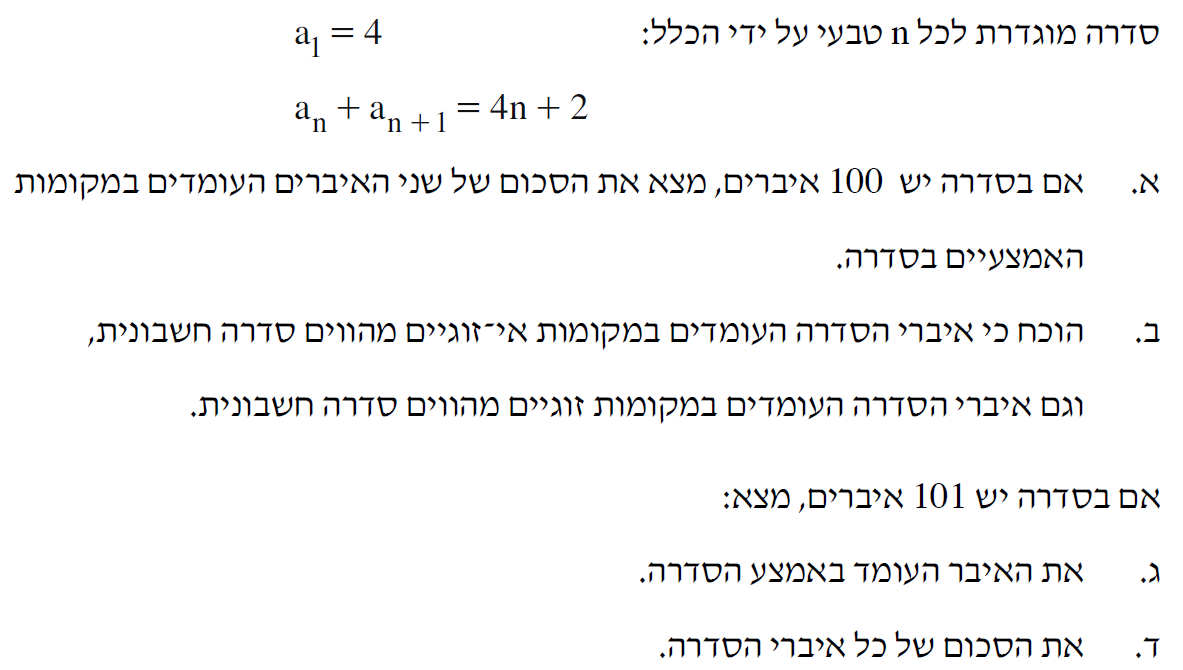
\includegraphics[width=.8\textwidth]{winter-2015-2}
\end{center}

\paragraph{סעיף א}
סכום שני איברי האמצע לפי הנוסחה הנתונה:
\begin{eqnarray*}
a_{50} + a_{51} &=& 4n+2\\
&=&4\cdot 50 +2\\
&=& 202\,.
\end{eqnarray*}

\vspace{-4ex}\paragraph{סעיף ב}

סדרה היא חשבונית אם ההפרש בין שני איברים עוקבים קבוע ולא תלוי ב-
$n$.

לאיברים הזוגיים:
\begin{eqnarray*}
a_{2k+2} - a_{2k} &=& a_{2k+2} + a_{2k+1} - a_{2k+1} - a_{2k}\\
&=& (a_{2k+1} + a_{2k+2}) - (a_{2k} + a_{2k+1})\\
&=&(4(2k+1)+2) - (4(2k)+2))\\
&=&8k+4+2-8k-2\\
&=&4\,.
\end{eqnarray*}
לאיברים האי-זוגיים:
\begin{eqnarray*}
a_{2k+3} - a_{2k+1} &=& a_{2k+3} + a_{2k+2} - a_{2k+2} - a_{2k+1}\\
&=& (a_{2k+2} + a_{2k+3}) - (a_{2k+1} + a_{2k+2})\\
&=&(4(2k+2)+2) - (4(2k+1)+2))\\
&=&8k+8+2-8k-4-2\\
&=&4\,.
\end{eqnarray*}

\paragraph{סעיף ג}
אם לסדרה
$101$
איברים, האיבר באמצע הסדרה הוא
$a_{51}$
שהוא מספר במקום אי-זוגי בסדרה, וניתן לחשב אותו לפי הנוסחה
$a_n=a_1+(n-1)d$
כאשר הנוסחה מתייחסת רק לסדרת האיברים במקומות האי-זוגיים
$1\leq k \leq 26, b_{2(k-1)+1}$:
\[
b_1 = a_{2\cdot 0+1}=a_1, \;\; b_2 = a_{2\cdot 1+1}=a_3, \;\;\ldots,\;\; b_{26} = a_{2\cdot 25+1}=a_{51}\,.
\]
לכן:
\[
a_{51}=b_{26}=b_1 + (k-1)\cdot d = 4 + 25\cdot 4 = 104\,.
\]

\vspace{-4ex}\paragraph{סעיף ד}

מהנוסחה לסכום של סדרה חשבונית:
\[
S = \frac{101}{2}(2\cdot 4 + (101-1)\cdot 4) = \frac{101}{2}\cdot 408 = 20604\,.
\]

\vspace{-4ex}\paragraph{שגיאה!}
הוכחנו שהאיברים הזוגיים הם סדרה חשבונית והאיברים האי-זוגיים הם סדרה חשבונית, אבל לא הוכחנו \textbf{שכל} האיברים הם סדרה חשבונית אחד. אם בודקים מספר איברים מתחילת הסדרה נראה מיד שהסדרה כולה אינה חשבונית:
\selectlanguage{english}
\begin{equation}
4, \raisebox{1ex}{$2$}, 8, \raisebox{1ex}{$6$}, 12, \raisebox{1ex}{$10$}, 16, \raisebox{1ex}{$14$}, \ldots \label{e.even-odd}
\end{equation}
\selectlanguage{hebrew}
המספרים הזוגיים מופיעים מעט גבוה יותר כדי להדגיש שתת-הסדרות הן סדרות חשבוניות אבל הסדרה כולה אינה חשבונית.

הפתרון הוא לסכם את כל אחת משתי הסדרות בנפרד ולחבר את הסכומים:
\[
\begin{array}{lll}
S_{\mathit{odd}}&=&\frac{51}{2}(2\cdot 4 + 50\cdot 4) = \frac{51}{2}\cdot 208=5304\\
\\
S_{\mathit{even}}&=&\frac{50}{2}(2\cdot 2 + 49\cdot 4) = \frac{50}{2}\cdot 200=5000\\
\\
S_{\mathit{odd}}+S_{\mathit{even}}&=&10304\,.
\end{array}
\]

\vspace{-4ex}\paragraph{מסקנות}

\begin{itemize}
\item
אין בהכרח קשר בין סדרה לבין תת-הסדרות שלה, לכן יש להקפיד על קריאה מדוייקת של השאלה כדי לוודא באיזו סדרה מדוברת. כאן ראינו שסדרה המורכבת משתי סדרות חשבוניות אינה בהכרח חשבונית. ההיפך גם נכון. נתון הסדרה החשבונית:
\[
a_1=2, a_2=4, a_3=6, a_4=8, a_5=10, a_6=12, a_7=14, a_8=16, \ldots
\]
תת-הסדרה $a_n$ כאשר $n$ הוא מספר ראשוני היא לא סדרה חשבונית:
\[
a_2=4, a_3=6, a_5=10, a_7=14, a_{11}=22, a_{13}=26,\ldots
\]
\vspace{-4ex}
\item
 יש להקפיד בניסוחים להבדיל בין איברי הסדרה ומקומותיהם בסדרה. במדעי המחשב משתמשים במונח קצר וברור
\L{index}
לתיאור מקום בסדרה.
\item
בשאלות על סדרות כדאי לרשום מספר איברים מתחילת הסדרה כדי לקבל מבט  כללי על הסדרה. סדרת המספרים ב-
\L{(\ref{e.even-odd})}
מראה בצורה ברורה שהסדרה המקורית אינה חשבונית.
\end{itemize}

\newpage

%%%%%%%%%%%%%%%%%%%%%%%%%%%%%%%%%%%%%%%%%%%

\section*{קיץ תשע"ה מועד ב, שאלה 2}

\begin{center}
\selectlanguage{english}
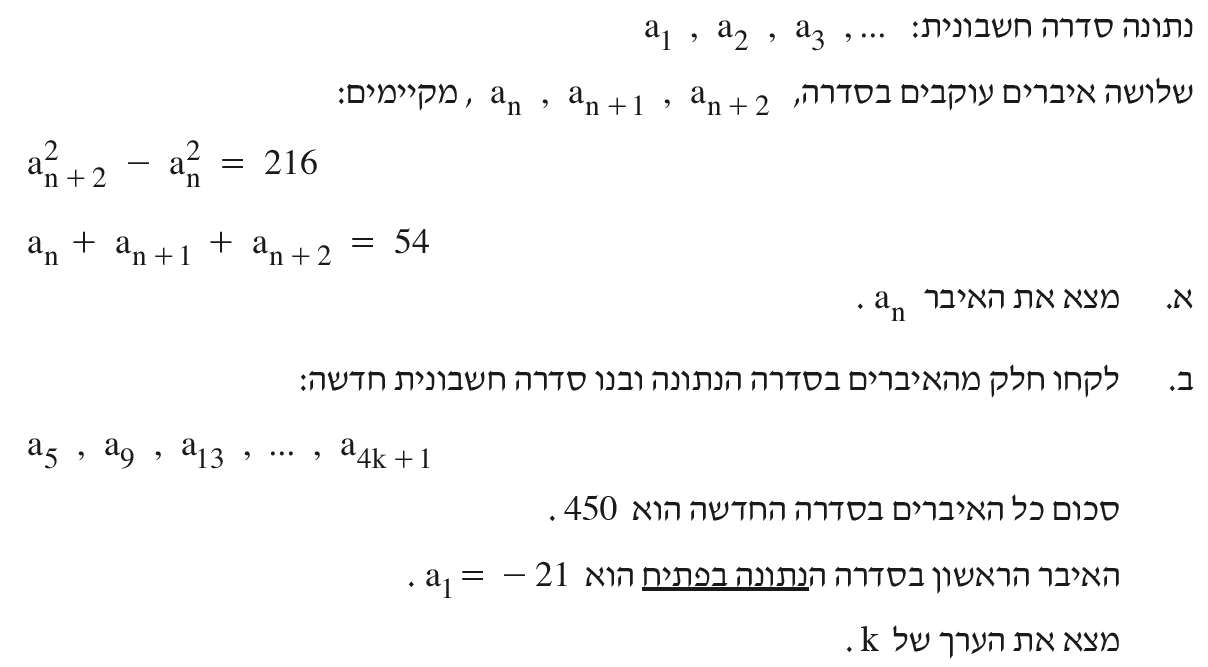
\includegraphics[width=.8\textwidth]{summer-2014b-2}
\end{center}

\vspace{-4ex}\paragraph{סעיף א}
ניתן לבטא את הערכים של איברים עוקבים על ידי הוספת ההפרש לאיבר הראשון:
\[
a_{n+1} = a_n + d, \; a_{n+2} = a_n + 2d\,.
\]
מהנוסחה הנתונה הראשונה:
\begin{eqnarray*}
a^2_{n+2} - a^2_n &=& 216\\
(a_n + 2d)^2 - a^2_n &=& 216\\
a_n^2 + 2a_nd + 4d^2 - a^2_n &=& 216\\
2a_nd + 4d^2 &=& 216\\
a_nd + 2d^2 &=& 108\,.
\end{eqnarray*}
מהנוסחה הנתונה השנייה:
\begin{eqnarray*}
a_n + a_{n+1} + a_{n+2} &=& 54\\
a_n + a_n + d + a_n + 2d &=& 54\\
3a_n + 3d &=& 54\\
a_n &=& \frac{54-3d}{3}\\
a_n &=& 18-3d\,.
\end{eqnarray*}
אם נציב את הביטוי עבור $a_n$ במשוואה הראשונה נקבל משוואה ריבועית ב- $d$:
\begin{eqnarray*}
(18-3d)d + 2d^2 &=& 108\\
18d-3d^2+2d^2-108&=&0\\
-d^2 + 18d - 108 = 0
\end{eqnarray*}
שפתרונה היא:
\[
d = \frac{-18 \pm \sqrt{324-432}}{-2}\,.
\]

\vspace{-4ex}\paragraph{שגיאה!}

הביטוי בשורש לא יכול להיות שלילי. החשד המיידי הוא שגיאה בחישובים ואכן יש כאן שתיים. השגיאה הראושנה היא טעות במכפלה:
\begin{eqnarray*}
a^2_{n+2} - a^2_n &=& 216\\
(a_n + 2d)^2 - a^2_n &=& 216\\
a_n^2 + 4a_nd + 4d^2 - a^2_n &=& 216\\
4a_nd + 4d^2 &=& 216\\
a_nd + d^2 &=& 54\,.
\end{eqnarray*}
השגיאה השנייה גם היא טעות פשוטה בחישוב:
\begin{eqnarray*}
a_n + a_{n+1} + a_{n+2} &=& 54\\
a_n + a_n + d + a_n + 2d &=& 54\\
3a_n + 3d &=& 54\\
a_n + d &=& 18\,.
\end{eqnarray*}
מההצבה מקבלים תוצאה הגיונית:
\begin{eqnarray*}
(18-d)d + d^2 &=& 54\\
18d - d^2 + d^2 &=& 54\\
18d &=& 54\\
d &=& 3\,.
\end{eqnarray*}
שים לב שלא גמרנו לפתור את השאלה שביקשה את ערכו של $a_n$:
\[
a_n=18-d=18-3=15\,.
\]

\vspace{-4ex}\paragraph{סעיף ב}
נחשב את האיבר
$a_5$:
\selectlanguage{english}
\begin{equation}
a_5 = a_1 + 4d = -21 + 4\cdot 3 = -21 + 12 = -9\,. \label{e.diff}
\end{equation}
\selectlanguage{hebrew}

נרשום את סדרת האיברים כדי לוודא שלא טעינו במקדם
$4$
של
$d$:
\[
a_1 = -21,\, a_2 = -18,\, a_3 = -15,\, a_4 = -12,\, a_5 = -9\,.
\]
בסדרה החדשה האינדקסים קופצים בהפרשים של
$4$
יחסית לסדרה המקורית. מהשוואה
\L{(\ref{e.diff})}
רואים שההפרש של הסדרה החדשה הוא
$4\cdot 3=12$,
אבל כדי לוודא נרשום את הסדרה:
\[
a_5 = -9,\, a_6 = -6,\, a_7 = -3,\, a_8 = -0,\, a_9 = 3\,,
\]
ואכן ההפרש בין
$-9$
ל
$3$
הוא 
$12$.

בסדרה החדשה, ניתן לרשום את האינדקס של האיבר הראשון כ-
$5 = 4\cdot 1+1$
והאינדקס של האיבר האחרון הוא
$4k+1$,
כך שיש 
$k$
איברים בסדרה השנייה.

סכום הסדרה החדשה נתונה ונשתמש בנוסחה לסכום הסדרה:
\begin{eqnarray*}
\frac{k}{2}(2\cdot -9 + (k-1)\cdot 12) &=& 450\\
\frac{k}{2}(-18+12k-12) &=& 450\\
6k^2 -15k - 450 &=&0\\
2k^2 -5k - 150 &=&0\,.
\end{eqnarray*}
פתרון המשוואה הריבועית:
\[
k=\frac{5\pm \sqrt{25+8\cdot 150}}{4} = \frac{5\pm 35}{4}= \frac{40}{4} = 10
\]
כי מספר האיברים חיובי.

\paragraph{מסקנות}

\begin{itemize}
\item
אין מנוס מבדיקת החישובים שוב ושוב. בדוק את החישובים מייד, לאחר סיום הפתרון, ואם יש זמן לאחר השלמת הבחינה.
\item
שימוש במחשבון לא פותר מבדיקת החישובים כי טעויות בהקלדה הן שכיחות כמו טעויות בחישוב.
\item
מומלץ "לבזבז" עוד כמה שניות כדי לרשום חישובים לפרטי פרטים. אני חישבתי ריבוע של ביטוי בראש ויכול להיות שכתיבת הריבוע כמכפלה היתה מונעת את הטעות:
\[
(a_n+2d)^2 - a_n^2 = (a_n+2d)(a_n+2d) - a_n^2\,.
\]
מאותה סיבה, כדאי לפשט משוואות לפני שפותרים אותן:
\begin{eqnarray*}
3a_n + 3d &=& 54\\
a_n + d &=& 18\,.
\end{eqnarray*}
זה נחמד אם אתה זוכר ש-
$54$
מתחלק ב-
$3$,
אבל גם אם לא, כדאי לבדוק בחילוק או אפילו במחשבון כי יש פחות סיכוי לטעות עם מספרים קטנים.

\item
אפשרות אחרת היא לפרק את הפולינום:
\[
a^2_{n+2} - a^2_n = (a_{n+2} - a_n)(a_{n+2}+a_n)\,.
\]
הצבה של
$a_{n+2}=a_n+2d$
מובילה מיד לפתרון. אכן, ראיתי תלמידים רבים המסרבים לבדוק פירוק של פולינומים, גם כאשר הפירוק יכול לספק הבנה טובה של חישוב.
\end{itemize}

\newpage

%%%%%%%%%%%%%%%%%%%%%%%%%%%%%%%%%%%%%%%%%%%

\section*{חורף תשע"ה, שאלה 3}

\begin{center}
\selectlanguage{english}
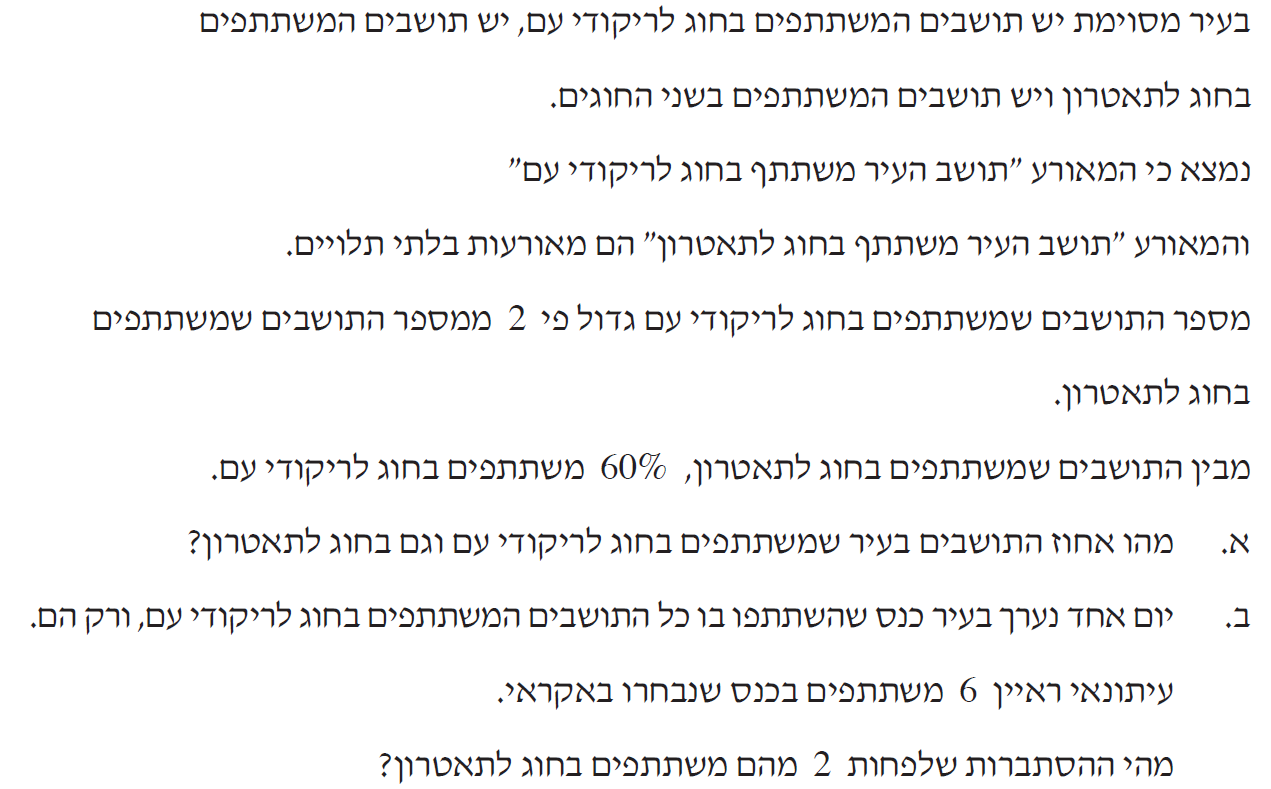
\includegraphics[width=.8\textwidth]{winter-2014-3}
\end{center}

אתחיל עם פתרון נכון ואחר כך אציג פתרון חלופי שגוי.

\bigskip

\textbf{\R{פתרון ראשון}}

\vspace{-2ex}\paragraph{סעיף א}

נסמן ב-$A$ את האירוע של משתתף בחוג לריקודי עם וב-$T$ את האירוע של משתתף בחוג לתיאטרון. $x$ הוא ההסתברות של האירוע $T$ ולפי המידע הנתון, ההסתברות של האירוע $A$ הוא $2x$:


\begin{center}
\renewcommand{\arraystretch}{1.2}
\setlength{\tabcolsep}{12pt}
\begin{tabular}{|c|c|c|c|}
\hline
&$\overline{T}$&$T$&\\\hline
$2x$&&$p(A\cap T)$&$A$\\\hline
&&&$\overline{A}$\\\hline
$1$&&$x$&\\\hline
\end{tabular}
\end{center}

לפי המידע הנתון, כולל הקביעה שהאירועים בלתי תלויים:

\[
.6 \cdot p(T) = p(A\cap T) = P(A) \cdot P(T)\,.
\]
לכן:
\begin{eqnarray*}
0.6x &=& 2x \cdot x\\
0.6 &=& 2x\\
x &=& 0.3
\end{eqnarray*}

נרשום ערכים מספריים בטבלה:

\begin{center}
\renewcommand{\arraystretch}{1.2}
\setlength{\tabcolsep}{12pt}
\begin{tabular}{|c|c|c|c|}
\hline
&$\overline{T}$&$T$&\\\hline
$0.6$&&$0.18$&$A$\\\hline
$0.4$&&&$\overline{A}$\\\hline
$1$&$0.7$&$0.3$&\\\hline
\end{tabular}
\end{center}

תשובה לסעיף זה של השאלה היא
$18\%$.

\vspace{-1ex}\paragraph{סעיף ב}

אנו צריכים עכשיו את ההסתברות המותנית כי בוחרים מתוך המשתתפים בריקודי עם:
\[
p(T / A) = \frac{p(T\cap A)}{p(A)} = \frac{0.18}{0.6} = 0.3\,,
\]
או:
\[
p(T / A) = \frac{p(T\cap A)}{p(A)} = \frac{p(T)p(A)}{p(A)} = p(T) = 0.3\,.
\]

מנוסחת ברנולי נקבל את ההסתברות של לפחות שני משתתפים בחוג לתיארטון כאחד פחות ההסתברות של אפס או אחד משתתפים בחוג לתיאטרון:

\[
1 - \left(\begin{array}{c}6\\0\end{array}\right) (0.3^0) (0.7^6) - \left(\begin{array}{c}6\\1\end{array}\right) (0.3^1) (0.7^5) = 1-0.1176-0.3025 = 0.57987\,.
\]

\vspace{-1ex}\paragraph{פתרון שני}

פרט לקביעה שהאירועים בלתי-תלויים, הבעיה מנוסחת כבעיה על קבוצות ולא כבעיה בהסתברות, לכן ניסיתי לפתור בצורה אחרת. נסמן:

מספר המשתתפים
\textbf{רק}
בחוג ריקודי עם = A.

מספר המשתתפים
\textbf{רק}
בחוג לתיאטרון = T.

מספר המשתתפים
\textbf{בשני החוגים}
= S.

מכאן שמספר המשתתפים בריקודי עם הוא $A+S$ ומספר המשתתפים בתיאטרון הוא $T+S$. לפי המידע בבעיה:
\begin{eqnarray*}
A + S &=& 2(T + S)\\
A &=& 2T + S\\
0.6(T+S) &=& S\\
T &=& \frac{S-0.6S}{0.6} = \frac{2}{3} S\\
A &=& 2\cdot \frac{2}{3} S + S = \frac{7}{3}S
\end{eqnarray*}
החלק של התושבים המשתתפים בשני החוגים הוא:
\[
\frac{S}{S+A+T} = \frac{S}{S+\frac{7}{3}S+\frac{2}{3}S} = \frac{3}{12}\,,
\]
והתשובה היא $25\%$.

\paragraph{מה הבעיה עם הפתרון?}

התוצאה חשודה כי לא השתמשנו במידע שהאירועים בלתי תלויים. הבעיה היא בהנחה
\textbf{\R{שכל}} 
התושבים משתתפים בלפחות חוג אחד. אם מסתכלים שוב על הטבלה, חסר נתון למשבצת
$\overline{A}\cap\overline{T}$.
אם יש תושבים שלא משתתפים בחוגים, יש נעלם נוסף וצריכים להשתמש במידע על אירועים בלתי-תלויים, וזה מחזיר אותנו לפתרון על ידי הסתברות ולא קבוצות.

מה מקור ההנחה? ניתן לפרש את המשפט הראשון בשאלה כך שהוא מפרט את עיסוקם של כל תושבי בעיר.

\paragraph{מסקנות}

אסור להניח שתיאור של קבוצות מכסה את כל המרחב אלא אם כתוב כך במפורש. למשל, בסעיף ב' כתוב: כל התושבים המשתתפים בחוג לריקודי עם,
\textbf{\R{ורק הם}}.



\newpage

%%%%%%%%%%%%%%%%%%%%%%%%%%%%%%%%%%%%%%%%%%%

\section*{קיץ תשע"ד מועד ב, שאלה 3}

\begin{center}
\selectlanguage{english}
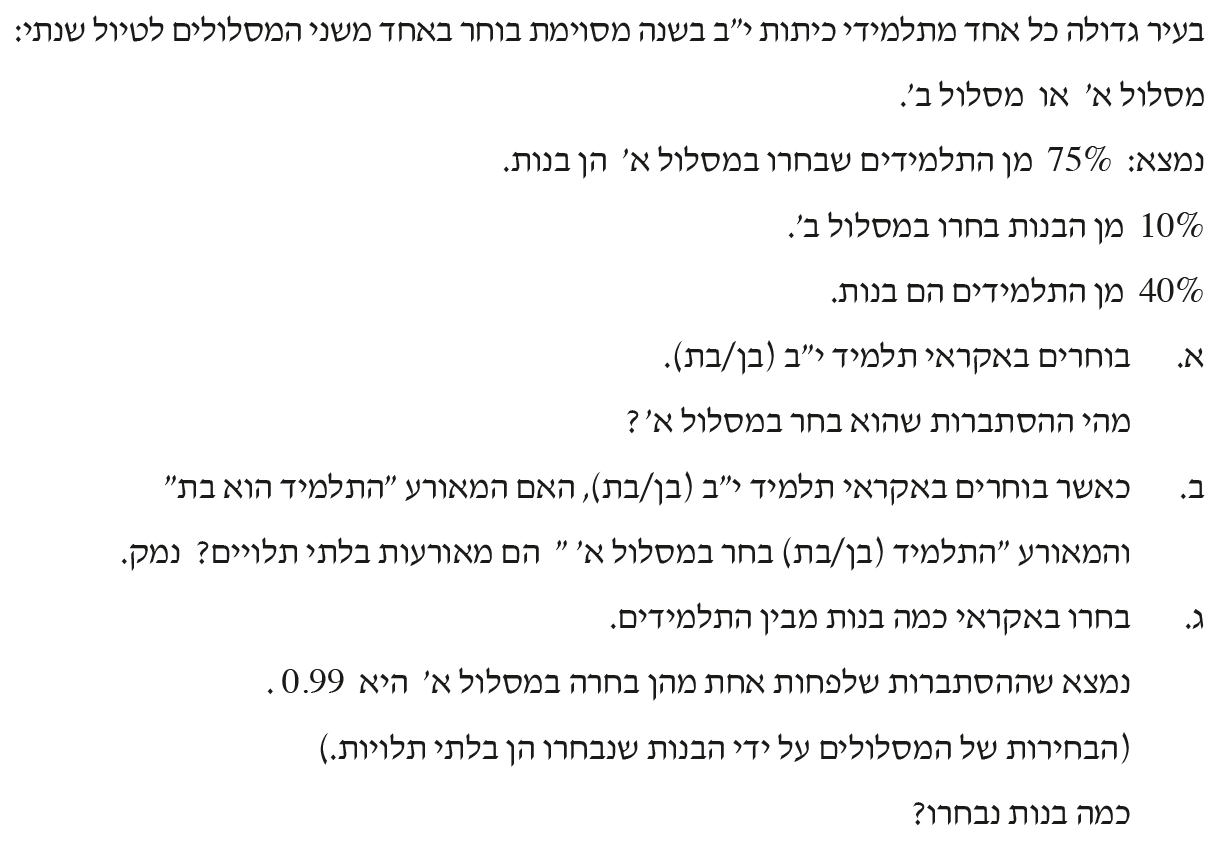
\includegraphics[width=.8\textwidth]{summer-2014b-3}
\end{center}

\vspace{-4ex}\paragraph{סעיף א}

בונים עץ לפי המידע בשאלה:
\begin{center}
\selectlanguage{english}
\begin{tikzpicture}[inner sep=0pt,node distance = 1cm and 2.5cm]
\node (root) {};
\node (bat) [below left=of root] {};
\draw (root) -- node[left,xshift=-4mm] { $0.4=$
\R{בת}
} (bat);
\node (boy) [below right=of root] {};
\draw (root) -- node[right,xshift=3mm] { $0.6=$
\R{בן}
} (boy);

\node (bbat) [below left=1cm of bat] {};
\draw (bat) -- node[left,xshift=-3mm] { $0.1=$
\R{ב}
} (bbat);
\node (abat) [below right=1cm of bat] {};
\draw (bat) -- node[right,xshift=3mm] { $0.75=$
\R{א}
} (abat);

\node (bboy) [below left=1cm of boy] {};
\draw (boy) -- node[left,xshift=-3mm] { $0.9=$
\R{ב}
} (bboy);
\node (aboy) [below right=1cm of boy] {};
\draw (boy) -- node[right,xshift=3mm] { $0.25=$
\R{א}
} (aboy);

\node (ag) [below=1mm of abat] {$\surd$};
\node (ab) [below=1mm of aboy] {$\surd$};
\end{tikzpicture}
\end{center}

ההסתברות שתלמיד בוחר מסלול א' מתקבלת מסכום ההסתברויות המסומנות:
\[
0.4 \times 0.75 + 0.6 \times 0.25 = 0.45\,.
\]

\vspace{-6ex}\paragraph{שגיאה!}
רואים שהעץ לא הגיוני כי כאשר יוצאים שני צאצאים מצומת, סכום ההסתברויות צריך להיות אחד. מקור הטעות הוא בקריאה לא נכונה של המשפט:
$75\%$
מן התלמידים שבחרו במסלול א' הן בנות. פירשתי את ההסתברות המותנית בצור
הפוכה כאילו שזה אחוז התלמידות שבחרו במסלול א'.

\vspace{-2ex}\paragraph{פתרון א}
נשתמש בנוסחה להסתברות מותנית:
\[
p(\textit{bat} \cap \textit{aleph}) =
p(\textit{bat} / \textit{aleph}) p(\textit{aleph}) =
p(\textit{aleph} / \textit{bat}) p(\textit{bat})\,.
\]
ומכאן:
\[
p(\textit{aleph}) = \frac{p(\textit{aleph} / \textit{bat}) p(\textit{bat})}{p(\textit{bat} / \textit{aleph})}= \frac{(1-0.1)\times 0.4}{0.75} = 0.48\,.
\]

\vspace{-2ex}\paragraph{פתרון ב}
נשתמש בנוסחה להסתברות מותנית בשני שלבים:
\[
0.1 = p(\textit{bet}/\textit{bat}) = \frac{p(\textit{bet}\cap\textit{bat})}{p(\textit{bat})} = \frac{p(\textit{bet}\cap\textit{bat})}{0.4}\,,
\]
\[
p(\textit{bet}\cap\textit{bat}) = 0.1 \times 0.4 = 0.04
\]
נציב בטבלה את הערכים הידועים והערך שחישבנו:
\begin{center}
\renewcommand{\arraystretch}{1.2}
\setlength{\tabcolsep}{12pt}
\begin{tabular}{|c|c|c|c|}
\hline
&bat&ben&\\\hline
aleph&$0.36$&&\\\hline
bet&$0.04$&&\\\hline
&$0.4$&$0.6$&$1$\\\hline
\end{tabular}
\end{center}
ונקבל ש-
$p(\textit{bat}\cap\textit{aleph})=0.36$.
נשתמש שוב בנוסחה להסתברות מותנית:
\[
p(\textit{bat}/\textit{aleph}) = \frac{p(\textit{bat}\cap\textit{aleph})}{p(\textit{aleph})}\,,
\]
ונקבל:
\[
p(\textit{aleph}) = \frac{p(\textit{bat}\cap\textit{aleph})}{p(\textit{bat}/\textit{aleph})} = \frac{0.36}{0.75} = 0.48\,.
\]
הפתרון הראשון נראה פשוט יותר אבל השני יכול להתאים למי שרגיל לעבוד עם טבלאות.

\vspace{-2ex}\paragraph{סעיף ב}

עם הפתרון ש-
$p(\textit{aleph})=.48$
נוכל להשלים את הטבלה:
\begin{center}
\renewcommand{\arraystretch}{1.2}
\setlength{\tabcolsep}{12pt}
\begin{tabular}{|c|c|c|c|}
\hline
&bat&ben&\\\hline
aleph&$0.36$&$0.12$&$0.48$\\\hline
bet&$0.04$&$0.48$&$0.52$\\\hline
&$0.4$&$0.6$&$1$\\\hline
\end{tabular}
\end{center}
נחשב:
\begin{eqnarray*}
p(\textit{aleph}\cap \textit{bat})&=&0.36\\
p(\textit{aleph}) p(\textit{bat})&=&0.48\times 0.4 = 0.192\,,
\end{eqnarray*}
והמאורעות אינם בלתי תלויים.

\vspace{-1ex}\paragraph{סעיף ג}

אם נבחר בת אחת ההסתברות שהיא בחרה מסלול א' היא:
$p(\textit{aleph}\cap \textit{bat})=0.36$.

ההסתברות שלפחות בת אחת מתוך שתיים בחרה מסלול א' היא:
\[
\left(\begin{array}{c}2\\1\end{array}\right) 0.36 \times (1-0.36) +
\left(\begin{array}{c}2\\2\end{array}\right) 0.36 \times 0.36 = 0.46+0.13=0.59\,.
\]

\vspace{-6ex}\paragraph{שגיאה!}
בחרו רק בנות ולכן מדובר בהסתברות מותנית:
\[
p(\textit{bet} / \textit{bat}) = 0.1, \; p(\textit{aleph} / \textit{bat}) = 0.9\,.
\]
\vspace{-2ex}\paragraph{פתרון א}
בת אחת מתוך אחת בחרה מסלול א':
$0.9$.

נבדוק תחילה מה ההסתברות שלפחות בת אחת
\textbf{\R{מתוך שתיים}}
בחרה מסלול א'. מנוסחת ברנולי:
\[
\left(\begin{array}{c}2\\1\end{array}\right) 0.9 \times (1-0.9) +
\left(\begin{array}{c}2\\2\end{array}\right) 0.9 \times 0.9 = 0.18+0.81=0.99\,.
\]
ולכן מספר הבנות שנבחרו הוא
$2$.

\vspace{-2ex}\paragraph{פתרון ב}
עדיף לא לפתור בניסוי וטעיה אלא לזהות את הנעלם---מספר הבנות שנבחרו---ולמצוא משוואה עם הנעלם. ההסתברות שאף בת לא בחרה במסלול א' היא
$1-0.9=0.1$.
ההסתברות שאף בת מתוך $n$ בנות לא בחרה במסלול א' היא
$(0.1)^n$
ונתון שהסתברות זו היא
$1-0.99=0.01$.
מספר הבנות הוא פתרון המשוואה:
\[
(0.1)^n = 0.01\,,
\]
שהוא
$n=2$.

\vspace{-1ex}\paragraph{מסקנות}

\begin{itemize}
\item
בניסוח שאלות בהסתברות לא נאמר במפורש "הסתברות מותנית", ועליך להבין מתוך מילים כגון "מן", "מבין" שמדובר בהסתברות מותנית. מכאן יש לקרוא שאלות אלו במשנה זהירותכדי לוודא שהבנת נכון.
\item
צריך לשקול אם להשתמש בטבלה או בעץ או לוותר עליהם ולהסתפק בנוסחאות לבד. אם הפתרון לא יוצא בשיטה אחת כדאי לנסות שיטה אחרת.
\item
אמנם הנוסחה להסתברות מותנית והנוסחה של בייס נתונות, אבל אני מעדיף להסתכל עליהן ביחד כך:
\[
p(A / B) p(B) = p(A\cap B) = p(B/A) p(A)\,.
\]
אני מוצא שקל לזכור את הנוסחאות האלו וקל להציב ערכים ידועים כדי לפתור שאלה.
\item
בשאלה הדורשת לבחור פריט מתוך אוכלוסיה אפשר להעדיף שימוש בטבלה ולא בעץ.
\end{itemize}

\newpage

%%%%%%%%%%%%%%%%%%%%%%%%%%%%%%%%%%%%%%%%%%%

\section*{קיץ תשע"ד מועד ב, שאלה 4}

\begin{center}
\selectlanguage{english}
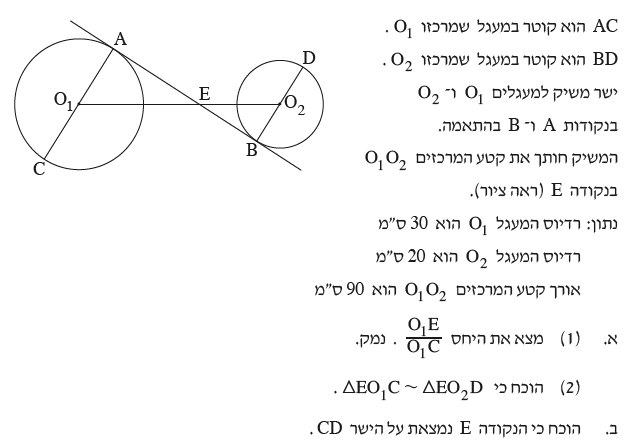
\includegraphics[width=.8\textwidth]{summer-2014b-4}
\end{center}

\vspace{-4ex}\paragraph{סעיף א}

\begin{center}
\selectlanguage{english}
\begin{tikzpicture}[scale=1.1]
\coordinate [label=left:$O_1$] (o1) at (0,0);
\coordinate [label=above:$A$] (A)  at (50:2);
\draw[rotate=-130] (A) rectangle +(4pt,4pt);
\coordinate [label=below:$C$] (C) at (-130:2);
\node [draw,circle through=(C)] at (o1) {};
\draw (A) -- (C);
\coordinate [label=right:$O_2$] (o2) at (5,0);
\coordinate [label=above:$D$] (D)  at ($(o2) + (50:1)$);
\coordinate [label=below:$B$] (B)  at ($(o2) + (-130:1)$);
\draw[rotate=50] (B) rectangle +(4pt,4pt);
\node [draw,circle through=(B)] at (o2) {};
\draw (B) -- (D);
\draw[name path=diameters] (o1) -- node[below,xshift=4mm] {\textsf{\small 90}} (o2);
\draw[name path=tangents] ($ (A) ! -.5 ! (B) $) -- ($ (A) ! 1.5 ! (B) $);
\path [name intersections={of=diameters and tangents,by={[label=above:$E$]E}}];
\path (A)  -- node[left] {\textsf{\small 30}} (o1);
\path (o1) -- node[left] {\textsf{\small 30}} (C);
\path (D)  -- node[right] {\textsf{\small 20}} (o2);
\path (o2) -- node[right] {\textsf{\small 20}} (B);
\path (o1) -- node[above] {$x$} (E);
\draw[dashed] (C) -- (D);
\end{tikzpicture}
\end{center}

\medskip

)1( הקו $AB$ משיק לשני המעגלים ולכן הזוויות
$\angle O_1 A E, \angle O_2 B E$
ישרות. הזוויות הקודקודיות
$\angle A E O_1, \angle B E O_2$
גם הן שוות. מכאן שהמשולשים
$\triangle O_1 A E, \triangle O_2 B E$
דומים. נסמן ב $x$ את הקטע
$O_1 E$
ונקבל את היחס:
\[
\frac{x}{30} = \frac{O_1 E}{O_1 A}= \frac{O_2 E}{O_2B} = \frac{90-x}{20}\,.
\]
נפתור את המשוואה עבור $x$ ונקבל
$50x = 2700$
ו 
$x=54$.
לכן:
\[
\frac{O_1 E}{O_1 C} = \frac{54}{30} = \frac{9}{5}\,.
\]
)2( המשיק $AB$ ניצב ל $AC,BD$ ולכן קווים אלה מקבילים, והזוויות המתחלפות
$\angle C O_1 E$, $\angle D O_2 E$
שוות. הזוויות הקודקודיות
$\angle O_1 E C, \angle O_2 E D$
גם שוות ולכן המשולשים דומים:
\[
\triangle E O_1 C \sim \triangle E O_2 D\,.
\]

\vspace{-6ex}\paragraph{סעיף ב}
\mbox{}\\

\textbf{\R{הפתעה ושגיאה!}}
ברור מהציור שהנקודה $E$ נמצאת על הקו $CD$, אבל מסתבר שצריך להוכיח את הטענה, ולכן ההוכחה הקודמת שגויה. למרות שהמשושלים
$\triangle O_1 E C, \triangle O_2 E D$
דומים, ייתכן שהזוויות
$\angle O_1 E C, \angle O_2 E D$
אינן זוויות קודקודיות.

אפשר לתקן את הוכחה על ידי שימוש בעובדה שהוכחנו בסעיף א ש
$\triangle O_1 A E \sim \triangle O_2 B E$.
ערכי הרדיוסים שווים ואנו מקבלים יחס:
\[
\frac{O_1 C }{O_2 D} = \frac{r_1}{r_2} = \frac{O_1 A}{O_2 B} = \frac{O_1 E}{O_2 E}\,,
\]
והדמיון בין המשולשים
$\triangle O_1 E C, \triangle O_2 E D$
נובע מהיחס בין שני צדדים והשווין של הזווית המתחלפות ביניהם
$\angle C O_1 E, \angle D O_2 E$.

נתבונן בזוויות סביב הנקודה
$E$:
\begin{center}
\selectlanguage{english}
\begin{tikzpicture}[scale=1.1]
\coordinate [label=left:$O_1$] (o1) at (0,0);
\coordinate [label=above:$A$] (A)  at (50:2);
\coordinate [label=below:$C$] (C) at (-130:2);
\node [circle through=(C)] at (o1) {};
\draw (A) -- (C);
\coordinate [label=right:$O_2$] (o2) at (5,0);
\coordinate [label=above:$D$] (D)  at ($(o2) + (50:1)$);
\coordinate [label=below:$B$] (B)  at ($(o2) + (-130:1)$);
\node [circle through=(B)] at (o2) {};
\draw (B) -- (D);
\draw[name path=diameters] (o1) -- (o2);
\draw[name path=tangents] ($ (A) ! -.1 ! (B) $) -- ($ (A) ! 1.1 ! (B) $);
\path [name intersections={of=diameters and tangents,by={[label=above:$E$]E}}];
\path (A)  -- (o1);
\path (o1) -- (C);
\path (D)  -- (o2);
\path (o2) -- (B);
\path (o1) -- (E);
\node[xshift=-20pt,yshift=7pt] at (E) {$\alpha$};
\node[xshift=20pt,yshift=-7pt] at (E) {$\alpha$};
\node[xshift=35pt,yshift=6pt] at (E) {$\beta$};
\node[xshift=-35pt,yshift=-6pt] at (E) {$\beta$};
\draw (C) -- (D);
\end{tikzpicture}
\end{center}
בגלל המשולשים הדומים 
$\triangle O_1 E C, \triangle O_2 E D$
ו
$\triangle O_1 A E \sim \triangle O_2 B E$
הזוויות המסומנות
$\alpha$
שוות וגם הזוויות המסומנות
$\beta$.
לפי נתוני השאלה,
$AB$
הוא קו ישר ולכן:
\[
\angle AED = 180^\circ - \alpha - \beta\,.
\]
מכאן ש
\[
\angle CED = 180^\circ - \alpha - \beta + \alpha + \beta = 180^\circ\,,
\]
ולכן
$CD$
קו ישר.


%עכשיו שאנו יודעים שהזוויות 
%$\angle O_1 E C, \angle O_2 E D$
%שוות והקטעים
%$O_1 E, E O_2$
%הם קטעים של קו ישר אחד )לפי הבנייה המקורית(, אפשר להסיק ש $E$ נמצא על הקו $CD$.

\vspace{-1ex}\paragraph{מסקנה}

לעולם אין לסמוך על ציור! 

\newpage

\paragraph{אין לסמוך על ציור}

\mbox{}

כדי להדגים את המלכודת הממתינה למי שמסתמך על ציור, אביא הוכחה 
\textbf{\R{שכל}}
משולש הוא משולש שווי שוקיים! בציור להלן $P$ היא נקודת החיתוך בין חוצה הזווית של
$\angle A$
 לבין האנך האמצעי של $BC$. $D,E,F$ הן נקודות החיתוך של האנכים מ $P$ אל הצלעות.
 
\begin{center}
\selectlanguage{english}
\begin{tikzpicture}[scale=1]
\coordinate (P) at (0,0);
\node[xshift=4mm,yshift=1mm] at (P) {$P$};
\coordinate [label=left:$B$] (B)  at (-2,-2);
\coordinate [label=right:$C$] (C)  at (4,-2);
\coordinate [label=above:$A$] (A)  at (-1,2);
\node[below,yshift=-12pt,xshift=2pt] at (A) {$\alpha$};
\node[below,yshift=-12pt,xshift=15pt] at (A) {$\alpha$};
\draw (A) -- (B);
\draw (A) -- (C);
\draw (B) -- (C);
\draw (A) -- (P);
\draw (B) -- (P);
\draw (C) -- (P);
\coordinate[label=left:$E$] (E) at ($ (A) ! .44 ! (B) $);
\draw[rotate=-100] (E) rectangle +(4pt,4pt);
\draw (P) -- (E);
\coordinate[label=right:$F$] (F) at ($ (A) ! .33 ! (C) $);
\draw[rotate=-132] (F) rectangle +(4pt,4pt);
\draw (P) -- (F);
\coordinate[label=below:$D$] (D) at ($ (B) ! .33 ! (C) $);
\draw (D) rectangle +(4pt,4pt);
\draw (P) -- (D);
\node[left] at ($ (A) ! .5 ! (E) $) {};
\node[left] at ($ (B) ! .5 ! (E) $) {};
\node[below] at ($ (B) ! .5 ! (D) $) {$a$};
\node[below] at ($ (C) ! .5 ! (D) $) {$a$};
\node[right,xshift=2pt] at ($ (A) ! .5 ! (F) $) {};
\node[right,xshift=2pt] at ($ (C) ! .5 ! (F) $) {};
\end{tikzpicture}
\end{center}
$AP$
הוא חוצה הזווית של הזווית
$\angle A$.
המשולשים
$\triangle APE, \triangle APF$
הם ישר זווית עם זוויות שוות וצלע $AP$ משותף כך שהם חופפים. $PD$ הוא אנך אמצעי כך ש 
$BD=DC$
ולכן המשולשים
$\triangle DPB, \triangle DPC$
חופפים. מכאן ש
$PB=PC$.
המשלושים
$\triangle EPB, \triangle FPC$
הם ישר זווית עם יתר שווה ולכן גם הם חופפים. ניתן להסיק ש
$AE+EB=AF+FC$
והמשולש
$\triangle ABC$
שווה שוקיים.

\medskip

ההוכחה נכונה ויחסית פשוטה, אז מה הבעיה? הבעיה היא שהציור אינו נכון! אם תבנו את הציור תוך מדידת הזווית
$\angle A$
ומציאת נקודת האמצע $D$, תגלו שהנקודות $P$ ו- $E$ או $F$ נמצאות
\textbf{\R{מחוץ}}
למשולש.

\newpage


%%%%%%%%%%%%%%%%%%%%%%%%%%%%%%%%%%%%%%%%%%%

\section*{חורף תשע"ד, שאלה 5}

\begin{center}
\selectlanguage{english}
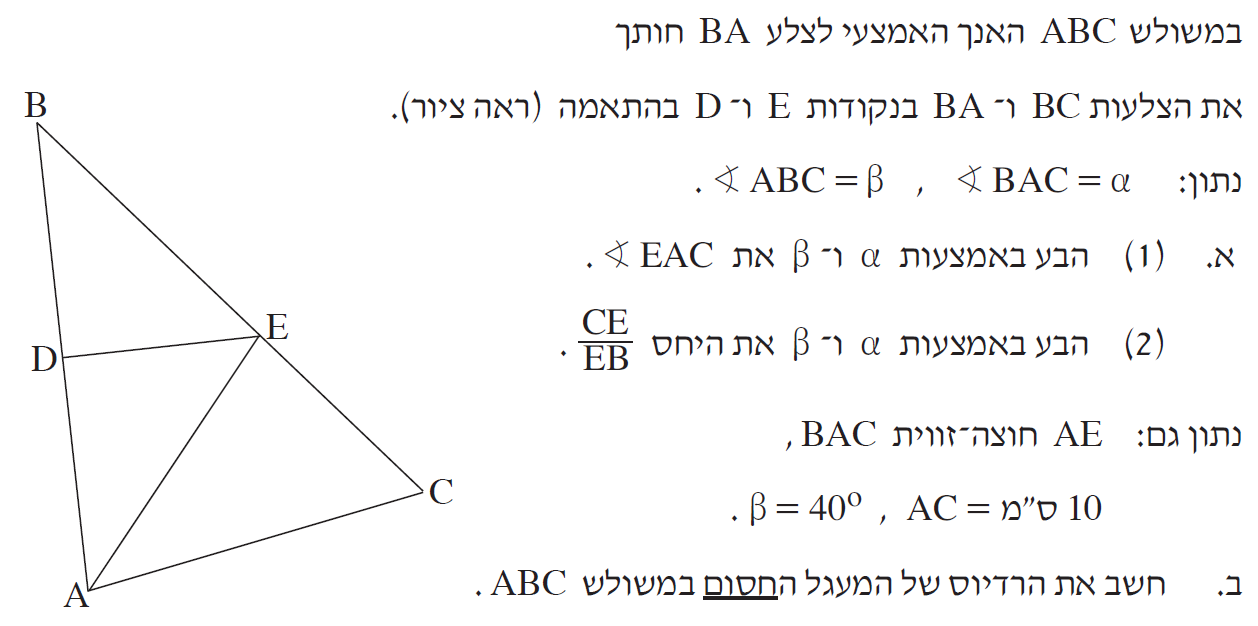
\includegraphics[width=.8\textwidth]{winter-2014-5}
\end{center}

\begin{center}
\selectlanguage{english}
\begin{tikzpicture}[scale=1.1]
\draw (0,0) coordinate (A) node[left] {$A$} -- (4,0) coordinate (C) node[right] {$C$} -- (1.5,5) coordinate (B) node[above] {$B$} -- cycle;
\coordinate [label=left:$D$] (D) at ($ (A) ! .5 ! (B) $);
\coordinate [label=right:$E$] (E) at ($ (B) ! .6 ! (C) $);
\draw (D) -- (E);
\draw[rotate=-105] (D) rectangle +(4pt,4pt);
\node[below,yshift=-4pt] at (B) {$\beta$};
\draw (6mm,0) arc [start angle=0, end angle=73, radius=6mm];
\node[above right,xshift=2pt] at (A) {$\alpha$};
\node[above right,yshift=14pt,xshift=8pt] at (A) {$\beta$};
\node[above right,yshift=-1pt,xshift=18pt] at (A) {$\alpha-\beta$};
\node[above right,yshift=6pt] at (C) {$180-(\alpha+\beta)$};
\draw[->] (4,.4) -- (3.6,.2);
\node[left] at ($ (A) ! .5 ! (D) $) {$a$};
\node[left] at ($ (B) ! .5 ! (D) $) {$a$};
\draw[dashed] (A) -- (E);
\node[right] at ($ (B) ! .5 ! (E) $) {$y$};
\draw[dashed] (A) %node[right,xshift=16pt,yshift=6pt] {$\gamma$}
-- node[above] {$y$} (E);
\end{tikzpicture}
\end{center}

\vspace{-4ex}\paragraph{סעיף א}
\mbox{}\\

)1( המשולשים
$\triangle ADE, \triangle BDE$
חופפים בגלל שני צלעות שווים והזווית )הישרה( ביניהם. לכן, הזווית
$\beta = \angle DAE$
והזווית
$\alpha - \beta = \angle EAC$.

דרך אחרת לראות את החפיפה היא לשים לב שהקטעים המסומנים
$y$
שווים כי הנקודה 
$E$
היא על האנך האמצעי ולכן במרחק שווה nקצות הקטע
$A,B$.

\medskip

)2( היתרים
$AE,EB$
שווים ומסומנים והזווית
$180 - (\alpha+\beta) = \angle ECA$.
לפי משפט הסינוסים במשולש
$\triangle ECA$:
\[
\frac{CE}{\sin (\alpha-\beta)}=\frac{AE}{\sin (180-(\alpha+\beta))}=\frac{EB}{\sin (180-(\alpha+\beta))}\,, 
\]
ולכן:
\[
\frac{CE}{EB}=\frac{\sin (\alpha-\beta)}{\sin 180-(\alpha+\beta)} =  \frac{\sin (\alpha-\beta)}{\sin (\alpha+\beta)}\,.
\]

\vspace{-4ex}\paragraph{סעיף ב}
\mbox{}\\

נתון 
$\angle ABC=\beta=40$
והוכחנו ש
$\angle BAE=\beta$.
נתון גם ש
$AE$
חוצה זווית כך ש
$\angle EAC=\angle BAE=40$.
במשולשים החופפים ישר-הזווית נקבל
$\angle BED=\angle AED=90-40=50$.
הזווית המשלימה
$\angle CEA$
היא
$180-50-50=80$
ולכן
$\angle ECA=180 - 80 - 40 =60$.

מרכז המעגל החסום במפגש של חוצי הזוויות. חוצה הזוית ב $C$ יפגוש את חוצה הזוית ב $A$: 
\begin{center}
\selectlanguage{english}
\begin{tikzpicture}
\draw (0,0) coordinate (A) node[left] {$A$} -- node[below] {$10$} (5,0) coordinate (C) node[right] {$C$} -- (2,1.5) coordinate (O) node[above] {$O$} -- cycle;
\node[above right,xshift=16pt] at (A) {$40$};
\node[above left,xshift=-24pt]  at (C) {$30$};
\node[below,xshift=2pt,yshift=-6pt] at (O) {$110$};
\end{tikzpicture}
\end{center}
נתון
$AC=10$
ולפי חוק הסינויסים:
\[
\frac{10}{\sin 110} = \frac{AO}{\sin 30}\,,
\]
\[
AO = \frac{10\sin 30}{\sin 100} = 5.3\,.
\]

\vspace{-4ex}\paragraph{שגיאה!}

רדיוס המעגל החסום הוא לא המרחק
$OA$
אלא הניצב $OF$ לצלע
$AC$,
כי
$AC$
הוא המשיק למעגל והניצב מהמרכז למשיק הוא הרדיוס.
\begin{center}
\selectlanguage{english}
\begin{tikzpicture}
\draw (0,0) coordinate (A) node[left] {$A$} -- (5,0) coordinate (C) node[right] {$C$} -- (2,1.5) coordinate (O) node[above] {$O$} -- cycle;
\draw[dashed] (O) -- (2,0) coordinate (F) node[below] {$F$};
\node[above right,xshift=16pt] at (A) {$40$};
\node[above left,xshift=-24pt]  at (C) {$30$};
\node[below,xshift=2pt,yshift=-6pt] at (O) {$110$};
\draw (F) rectangle +(4pt,4pt);
\end{tikzpicture}
\end{center}
החישוב פשוט:
\hspace{3em}
$OF = AO \sin 40 = 5.3\sin 40 = 3.4$.

\vspace{-2ex}\paragraph{מסקנות}
\begin{itemize}
\item
אי-אפשר להדגיש מספיק את החשיבות של קריאה מדוקדקת של השאלה במבחן. במיוחד חשוב להבין מה הפתרון הנדרש.
\item
מקרה אחר שנתקלתי בו היה דרישה לחשב את
\textbf{\R{כל}}
הזוויות במשולש ואין לעצור לאחר חישוב זווית אחת או שתיים אפילו שברור איך להשלים את הפתרון.
\item 
הייתי צריך לצייר את המעגל ואז הייתי רואה ש
$OF$
הוא הרדיוס.

\begin{center}
\selectlanguage{english}
\begin{tikzpicture}
\draw (0,0) coordinate (A) node[left] {$A$} -- (5,0) coordinate (C) node[right] {$C$} -- (2,1.5) coordinate (O) node[above] {$O$} -- cycle;
\draw[dashed] (O) -- (2,0) coordinate (F) node[below] {$F$};
\node [draw,circle through=(F)] at (O) {};
\draw (F) rectangle +(4pt,4pt);
\end{tikzpicture}
\end{center}

\end{itemize}

\newpage

%%%%%%%%%%%%%%%%%%%%%%%%%%%%%%%%%%%%%%%%%%%

\section*{חורף תשע"ד, שאלה 6}

\begin{center}
\selectlanguage{english}
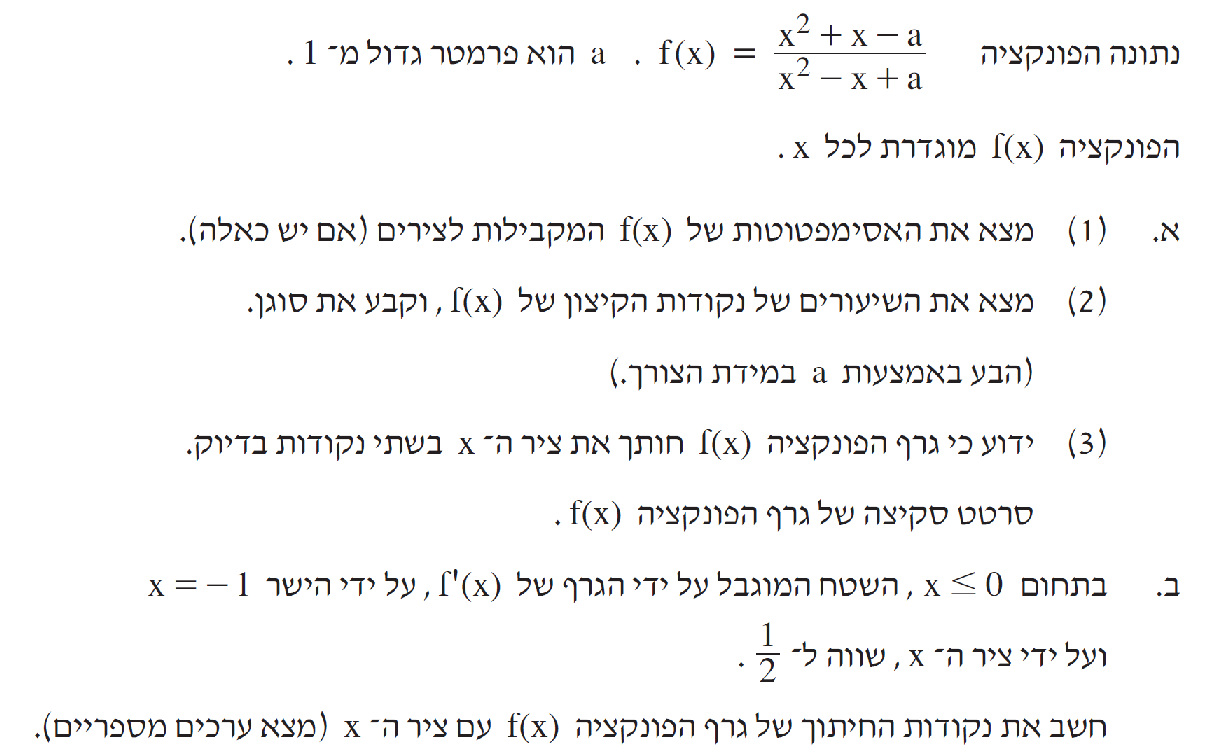
\includegraphics[width=.8\textwidth]{winter-2014-6}
\end{center}

א. )1( לא יכול להיות ש
$x^2-x+a=0$
כי
$a>1$
ותמיד
$x^2 \geq x$.
לכן אין אס' אנכיות.

נבדוק אס' אופקיות על ידי חילוק בגורם עם המעלה הגבוהה ביותר:
\[
\frac{1+\frac{1}{x}-\frac{a}{x^2}}{1-\frac{1}{x}+\frac{a}{x^2}}\,.
\]
כאשר
$\pm \infty \leftarrow x$,
$0 \leftarrow \frac{1}{x}, 0 \leftarrow \frac{a}{x^2}$,
והביטוי שואף ל
$1$.
מכאן שיש אס' אופקית ב
$y=1$.

\medskip

)2( הפונקציה מוגדרת לכל מספר ממשי לכן ייתכנו רק נקודות קיצון כאשר הנגזרת מתאפסת:
\[
f'(x) = \frac{(2x+1)(x^2-x+a)-(2x-1)(x^2+x-a)}{(x^2-x+a)^2} = 0\,.
\]
בהשמטת המכנה שהוא חיובי:
\begin{eqnarray*}
(2x^3 - 2x^2 +2xa + x^2 - x + a) -
(2x^3 + 2x^2 -2xa - x^2 - x + a) &=&0\\
-2x^2+4xa &=& 0\,.
\end{eqnarray*}
הנגזרת מתאפסת בנקודות:
\[
(0,-1), \left(2a,\frac{4a^2+a}{4a^2-a}\right)=\left(2a,\frac{4a+1}{4a-1}\right)\,.
\]
כדי לקבוע את סוג נקודות הקיצון, נבדוק את הסימן של הנגזרת השניה, ושוב ניתן להשמיט את המכנה החיובי של הנגזרת הראשונה כדי לקבל את הסימן של הנגזרת השנייה:
\[
(-2x^2+4ax)' = -4x + 4a.
\]
הביטוי חיובי כאשר 
$x=0$
ונקודת הקיצון היא מינימום. הביטוי שלילי כאשר
$x=2a$
ונקודת הקיצון היא מקסימום.

\medskip

\textbf{\R{שגיאה}}
קבלנו את התשובה הנכונה אבל הנימוק לא בהכרח נכון. חישוב הנגזרת של מנה הוא:
\[
\left(\frac{f}{g}\right)' = \frac{f'g - fg'}{g^2}\,.
\]
הפונקציה
$g$
מופיעה גם במונה ולא רק במכנה ואסור להשמיט אותה בחישוב הנגזרת השניה.

\medskip

הנה גרף של המונה של הנגזרת הראשונה 
$-2x^2+4ax$:
\begin{center}
\selectlanguage{english}
\begin{tikzpicture}[scale=.9,samples=20,domain=-.5:2.5]
\draw (-1,0) -- (3,0);
\draw (0,-1) -- (0,1);
\draw[fill] (0,0) circle [radius=1pt] node[above left] {$(0,0)$};
\draw[fill] (2,0) circle [radius=1pt] node[above right] {$(2a,0)$};
\draw plot (\x,{(-2*\x*\x+4*\x)/3});
\end{tikzpicture}
\end{center}
והנה הגרף של הנגזרת הראשונה:
\begin{center}
\selectlanguage{english}
\begin{tikzpicture}[scale=.9,samples=20,domain=-.5:3]
\draw (-1,0) -- (3,0);
\draw (0,-1) -- (0,1);
\draw[fill] (0,0) circle [radius=1pt] node[above left] {$(0,0)$};
\draw[fill] (2,0) circle [radius=1pt] node[above right] {$(2a,0)$};
\draw plot (\x,{(-2*\x*\x+4*\x)/(3*(\x*\x-\x+1)^2)});
\end{tikzpicture}
\end{center}
כצפוי צורת הגרף שונה אבל לא הנקודות בהן הנגזרת מתאפסת, ולכן גם לא המעבר של הנגזרת מחיובי לשלילי או משלילי לחיובי.

\medskip

הנגזרת השניה היא בעצם השיפוע של הנגזרת הראשונה, ואת זה ניתן לבדוק בחישוב השינוים בסימני הערכים סביב הערכים בהם הנגזרת הראשונה מתאפסת. )אנו מסתמכים על הרציפות של הפונקציה.( כדי לבדוק את שינוי הסימנים אכן אפשר להשמיט את המכנה:

\[
\renewcommand{\arraystretch}{1.2}
\setlength{\tabcolsep}{12pt}
\begin{array}{|c|r|r|r|r|r|}
\hline
x&-1&0&a&2a&3a\\\hline
-2x^2+4ax&-2-4a&0&2a^2&0&-6a^2\\\hline
&<0&0&>0&0&<0\\\hline
\end{array}\,.
\]
השיפוע חיובי ב
$0$
ויש כאן מינימום. השיפוע שלילי ב
$2a$
ויש כאן מקסימום.

\bigskip

)3( בגלל ש
$a>1$
נקודת הקיצון השניה נמצאת מעל לאס' 
$y=1$
ומכאן גרף הפונקציה הוא:
\begin{center}
\selectlanguage{english}
\begin{tikzpicture}[scale=.9,samples=50,domain=-4:4]
\draw (-4,0) -- (4,0);
\draw (0,-1.2) -- (0,2);
\coordinate (y) at (0,-1);
\draw[fill] (y) circle [radius=1pt] node[right,xshift=4pt] {$(0,-1)$};
\coordinate (x) at (2,1.67);
\draw[fill] (x) circle [radius=1pt] node[above] {$\left(2a,\frac{4a+1}{4a-1}\right)$};
\draw[dashed] (-4,1) -- (4,1);
\draw plot (\x,{(\x*\x+\x-1)/(\x*\x-\x+1)});
\end{tikzpicture}
\end{center}

\bigskip

ב. נתון תחום 
$x\leq 0$,
הישר
$x=-1$
וציר ה-$x$. חישוב השטח הוא:
\[
\frac{1}{2} = \int_{-1}^{0} f'(x) = \int_{-1}^{0} (-2x^2 + 4xa) dx\,.
\]

\textbf{\R{שגיאה}}
אנחנו רגילים לבדוק נקודות קיצין תוך התעלמות ממכנה חיובי. אבל כאן עלינו לבצע אינטגרציה של הנגזרת ולא רק של המונה שלו. בנוסף, האינטגרל של הנגזרת הוא הפונקציה הנתונה, כך שאין בכלל צורך בחישוב מייגע. 

\[
\frac{1}{2} = \int_{-1}^{0} f'(x) = f(0) - f(-1) = -1 - \frac{-a}{a+2} = \frac{-2}{a+2}\,.
\]
מפתרון המשוואה
$\frac{1}{2}=\frac{-2}{a+2}$
מקבלים
$a=-6$.

\medskip

\textbf{\R{שגיאה}}
נזכור שהשאלה קבעה ש
$a>1$.
אפשר גם שים לב ששטח לא יכול להיות שלילי. מעיון בגרף או מבדיקת כמה ערכים, נגלה שהנגזרת הראשונה שלילית כאשר 
$x<0$.
עלינו לבצע אניטגרציה לשלילת הפונקציה כדי לקבל:
\[
\frac{1}{2}=\int_{-1}^{0} -f'(x) = -f(0) + f(-1) = 1 + \frac{-a}{a+2} = \frac{2}{a+2}\,.
\]
מפתרון המשוואה
$\frac{1}{2}=\frac{2}{a+2}$
מקבלים
$a=2$.

\medskip

אמנם מצאנו את הערך של
$a$
אבל השאלה דרשה את נקודות החיתוך של 
$f(x)$
עם ציר ה-$x$. בגלל שהמכנה חיובי יש לחשב את ערכי $x$ בהם המונה מתאפס:
\begin{eqnarray*}
x^2+x-2 &=& 0\\
(x+2)(x-1) &=& 0
\end{eqnarray*}
ונקודות החיתוך הן 
$(-2,0), (1,0)$.
עיון בגרף מראה שהתשובה מתאימה.

\paragraph{מסקנות}

אי אפשר להפריז בחשיבות של קריאה מדוקדקת של השאלה ועבודה מסודרת:

\begin{itemize}
\item לקחנו רק את המונה של נגזרת במקום הנגזרת עצמה.
\item עצרנו בשמחה לאחר חישוב
$a$
בלי לשים לב שהשאלה דרשה נקודות חיתוך.
\item לפני חישוב שטח יש לבדוק אם השטח או חלקו נמצא מתחת לציר ה
$x$
ולהיערך בהתאם.
\item
לפעמים כותבי הבחינה מניחים סוכריות ולא רק מלכודות. כאן הם ביקשו לבצע אינטגרציה של נגזרת כאשר הפונקציה עצמה נתונה.
\end{itemize}

בבדיקה האם יש מינימום או מקסימום כאשר הנגזרת הראשונה מתאפסת, לא תמיד כדאי לחשב במפורש את הנגזרת השניה. אפשר לבדוק ערכים של הנגזרת הראשונה כדי לזהות את השיפועים.

\end{document}
